\documentclass[
    UTF8,
    twoside,
    zihao=5,
    scheme=plain,
    heading=true,
]{ctexrep}
\ctexset{
    %% section number depth - subsubsection
    secnumdepth=3,
    %% toc depth - subsection
    tocdepth = 2,
    chapter={
        nameformat={},
        titleformat={},
        name={},
        aftername={、},
        number={\chinese{chapter}},
        format={\bfseries \heiti \zihao{-4} \raggedright},
        beforeskip={0ex},
        afterskip={0.3ex},
    },
    section={
        aftername={、},
        number={\arabic{section}},
        format={\bfseries \songti \zihao{5} \raggedright},
        beforeskip={0.5ex},
        afterskip={0.5ex},
    },
    subsection={
      aftername={\quad},
      format={\bfseries \songti \zihao{5} \raggedright},
      afterskip={0.5ex},
      beforeskip={0.5ex},
    },
    subsubsection={
        aftername={\quad},
        format={\bfseries \songti \zihao{5} \raggedright},
        afterskip={0.5ex},
        beforeskip={0.5ex},
    }
}
\renewcommand{\figurename}{图}

\usepackage{geometry}
\geometry{
    a4paper,
    %margin=15mm,
    top=2.5cm,
    bottom=2.5cm,
    left=2.5cm,
    right=2.5cm
}
\usepackage{framed}
% \FrameSep0pt
\OuterFrameSep 0pt

% cite
% paper
\usepackage[style=ieee]{biblatex}
\addbibresource{ref.bib}
\newcommand{\upcite}[1]{\textsuperscript{\cite{#1}}}
% other
\RequirePackage[
    colorlinks=true,
]{hyperref}
\newcommand{\algorithmautorefname}{算法}
\renewcommand{\tableautorefname}{表}
\renewcommand{\figureautorefname}{图}
\newcommand{\subfigureautorefname}{图}
\renewcommand{\equationautorefname}{式}


\usepackage{indentfirst}

% math
%% symbol
\usepackage{amssymb,amsmath}
\newcommand{\vect}[1]{\boldsymbol{#1}} % vector
\newcommand{\mat}[1]{\mathbf{#1}}      % matrix
\newcommand{\tensor}[1]{\mathsf{#1}}   % tensor
\newcommand{\set}[1]{\mathbb{#1}}      % set
\newcommand{\T}{\mathrm{T}}            % transposition
\everymath{\displaystyle}              % block style 
%% environment
\usepackage{amsthm}
\theoremstyle{plain}
\newtheorem{theorem}{定理}[section]
\newtheorem{lemma}[theorem]{引理}
\newtheorem{proposition}[theorem]{命题}
\newtheorem*{corollary}{推论}
\theoremstyle{definition}
\newtheorem{definition}{定义}[section]
\newtheorem{conjecture}{猜想}[section]
\newtheorem{example}{例}[section]
\theoremstyle{remark}
\newtheorem*{remark}{\normalfont\heiti 评论}
\newtheorem*{note}{\normalfont\heiti 注}
\newtheorem{case}{\normalfont\heiti 案例}
\renewcommand*{\proofname}{\normalfont\heiti 证明}

\usepackage{setspace}
\usepackage{float}
\usepackage{pdfpages}
% table
\usepackage{array}
\usepackage{multirow}
\usepackage{makecell}
% checkbox
\usepackage{wasysym}

\begin{document}
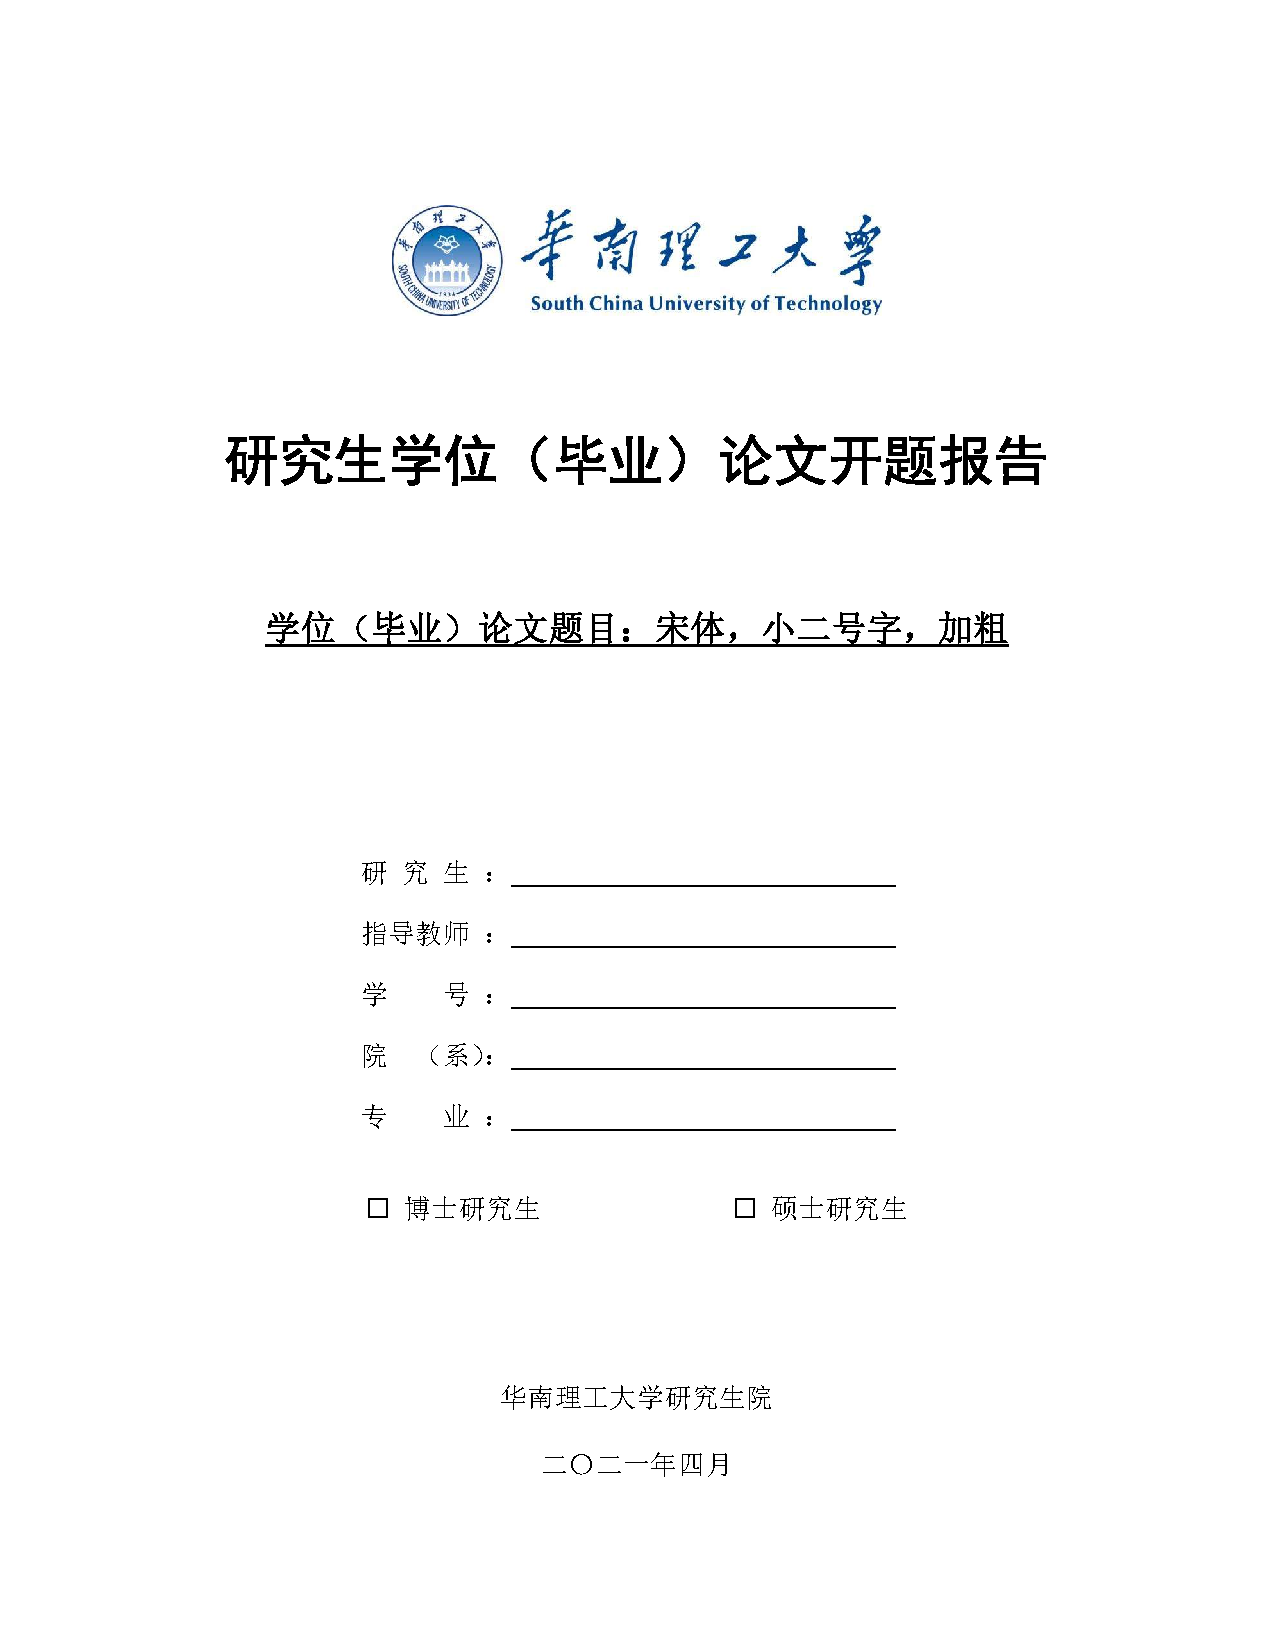
\includepdf[pages={1}]{cover.pdf}

\setcounter{page}{1}

\chapter{摘要}
\begin{table}[H]
  \renewcommand{\arraystretch}{1.5}
  \begin{tabular}{|ccl|}
  \hline
  \multicolumn{1}{|c|}{
    \multirow{2}{*}{
      \begin{tabular}[c]{@{}c@{}}
        论文\\ 题目
      \end{tabular}
      % \makecell[c]{论文\\ 题目}
    }
  } &
  \multicolumn{1}{c|}{中文} &
  \multicolumn{1}{c|}{中文题目}  \\ \cline{2-3} 
  \multicolumn{1}{|c|}{} &
  \multicolumn{1}{c|}{英文} &
  \multicolumn{1}{c|}{English title}  \\ \hline
  \multicolumn{2}{|c|}{
    \begin{tabular}[c]{@{}c@{}}
      论文选题项\\ 目是否涉密
    \end{tabular}
  } &
  \begin{tabular}[c]{@{}l@{}}
\Square 是,并已办理《华南理工大学学位论文定密审批表》审批手续,复印件已附于~\\本报告末页。\\
    \CheckedBox 否,并承诺学位论文将不涉及国家秘密和其他不宜公开的内容。
  \end{tabular}
  \\ \hline
  \multicolumn{2}{|c|}{
    \begin{tabular}[c]{@{}c@{}}
      摘\\要
    \end{tabular}
  } &
  \multicolumn{1}{l|}{
    \begin{tabular}[c]{@{}lp{3cm}@{}}
      % 手动填充
      ~\\~\\~\\~\\~\\~\\~\\~\\~\\~\\
      % 需要手动换行,使用 ~\\
      \quad \quad 摘要这里,这个模板有一个缺陷,就是下面这些文字,需要自己手动换行,~\\ 同时文字的上面也需要自己用换行来填充。具体怎么换行,你看一下 Latex 里~\\面怎么写就清楚了。~\\
      
      \quad \quad 所以我建议你把这一段要写的内容,都写完后,再来进行编辑如何换行。~\\如果有大佬来帮忙改进这个模板,十分感谢。欢迎各位来 PR。~\\

      % 手动填充
      ~\\~\\~\\~\\~\\~\\~\\~\\~\\~\\

    \end{tabular}
  }
  \\ \hline
  \multicolumn{1}{|c|}{
    \multirow{3}{*}{
      \begin{tabular}[c]{@{}c@{}}
        关\\ 键\\ 字
      \end{tabular}
    }
  } &
  \multicolumn{1}{c|}{中文} &
  关键字 1 \; 关键字 2 \; 关键字 3 \; 关键字 4 \\ \cline{2-3} 
  \multicolumn{1}{|c|}{} &
  \multicolumn{1}{c|}{英文} &
  keyword 1 / keyword 2 / keyword 3 / keyword 4 \\ \cline{2-3} 
  \multicolumn{1}{|c|}{} &
  \multicolumn{2}{l|}{
    1、关键词数量不少于三个;
    2、关键词之间空一格(英文用 / 分隔)
  }  \\ \hline
\end{tabular}
\end{table}

\newpage

\chapter{立题依据}

\begin{framed}
\begin{spacing}{1.5}
\section{研究意义}

填充你的内容

\section{国内外研究现状}

填充你的内容。

\section{主要参考文献及出处}

\printbibliography[heading=none]

\end{spacing}
\end{framed}
\newpage

\chapter{研究方案}

\begin{framed}
\begin{spacing}{1.5}

\section{研究目标、研究内容及拟解决的关键问题}

\subsection{研究目标}

填充你的内容

\subsection{研究内容}

填充你的内容

\subsection{关键问题}

填充你的内容

\section{拟采取的研究方法、技术路线及可行性分析}

填充你的内容

\section{创新之处}

填充你的内容

\end{spacing}
\end{framed}
\newpage

\chapter{研究条件与基础}

\begin{framed}
\begin{spacing}{1.5}

\section{相关的研究工作积累}

填充你的内容

\section{已具备的研究条件,尚缺少的研究条件和拟解决的途径}

填充你的内容

\newpage

\section{本人已取得的主要成果}

填充你的内容

\end{spacing}
\end{framed}

\newpage
\chapter{论文工作计划及预期成果}
\begin{table}[H]
  \renewcommand{\arraystretch}{2.1}
  \begin{tabular}{|lll|}
    \hline
    \multicolumn{3}{|l|}{论文工作进度安排}  \\ \hline
    \multicolumn{1}{|c|}{\makebox[2.7em][l]{\quad}起始时间\makebox[2.7em][l]{\quad}} &
    \multicolumn{1}{c|}{\makebox[9.6em][l]{\quad}工作内容\makebox[9.6em][l]{\quad}}  &
    \multicolumn{1}{c|}{\makebox[2.5em][l]{\quad}备注\makebox[2.5em][l]{\quad}} \\ \hline
    \multicolumn{1}{|l|}{2022.09-2023.02} & \multicolumn{1}{l|}{阅读文献并完成算法理论构建} &              \\ \hline
    \multicolumn{1}{|l|}{2023.02-2023.06} & \multicolumn{1}{l|}{编写相关代码并进行实验}    &              \\ \hline
    \multicolumn{1}{|l|}{2023.06-2023.08} & \multicolumn{1}{l|}{编写论文并投稿}           &              \\ \hline
    \multicolumn{1}{|l|}{}                & \multicolumn{1}{l|}{}                       &              \\ \hline
    \multicolumn{1}{|l|}{}                & \multicolumn{1}{l|}{}                       &              \\ \hline
    \multicolumn{1}{|l|}{}                & \multicolumn{1}{l|}{}                       &              \\ \hline
    \multicolumn{1}{|l|}{}                & \multicolumn{1}{l|}{}                       &              \\ \hline
    \multicolumn{1}{|l|}{}                & \multicolumn{1}{l|}{}                       &              \\ \hline
    \multicolumn{3}{|l|}{
      \begin{tabular}[c]{@{}l@{}}
        预期成果:\\ 1. 投稿相关论文一篇
      \end{tabular}
    }  \\ \hline
\end{tabular}
\end{table}

\newpage
\chapter{开题报告作者承诺及导师意见}
\begin{table}[H]
    \renewcommand{\arraystretch}{1.5}
    \begin{tabular}{|m{0.972\textwidth}|}
    \hline
    \begin{tabular}[c]{@{}l@{}}
      ~\\
      \quad \quad 我保证上述填报内容的真实性,并将在导师指导下,严格遵守学校的有关规定,按计划~\\
      认真开展学位(毕业)论文研究工作。\\~\\
      % 签名,可以自己加电子签名,或者不加手动写也行
      \makebox[20em][l]{\quad} 研究生(签名):
      
\includegraphics[width=6em]{img/person-signature.png}
      ~\\
      \makebox[26em][l]{\quad} \,2022 \, 年 \, 10 \, 月 \, 11 \, 日~\\
      ~\\
    \end{tabular} \\ \hline
    \begin{tabular}[c]{@{}l@{}}
      ~\\
      \quad \quad 我已审阅过开题报告的全部内容,同意参加开题报告会。~\\~\\
      \makebox[20em][l]{\quad} 指导老师(签名):
      
\includegraphics[width=4em]{img/supervisor-signature.png}
      ~\\
      \makebox[26em][l]{\quad} \,2022 \, 年 \, 10 \, 月 \, 11 \, 日~\\
      ~\\
    \end{tabular} \\ \hline
  \end{tabular}
\end{table}

\newpage
\chapter{开题报告审核意见}
\begin{table}[H]
  \renewcommand{\arraystretch}{2}
  \begin{tabular}{|clccc|}
  \hline
  \multicolumn{5}{|c|}{开题工作小组成员名单}  \\ \hline
  \multicolumn{2}{|c|}{\makebox[1.30em][l]{\quad}组成人员\makebox[1.30em][l]{\quad}} &
  \multicolumn{1}{c|}{\makebox[1.75em][l]{\quad}姓 \quad 名\makebox[1.75em][l]{\quad}} &
  \multicolumn{1}{c|}{\makebox[3.1em][l]{\quad}职 \quad 称\makebox[3.1em][l]{\quad}} &
  \multicolumn{1}{c|}{\makebox[5.73em][l]{\quad}工作单位\makebox[5.73em][l]{\quad}} \\ \hline
  \multicolumn{2}{|c|}{组长} & \multicolumn{1}{c|}{XX 1}   & \multicolumn{1}{c|}{教授}  & 华南理工大学 \\ \hline
  \multicolumn{2}{|c|}{成员} & \multicolumn{1}{c|}{XX 2}   & \multicolumn{1}{c|}{副教授}  & 华南理工大学 \\ \hline
  \multicolumn{2}{|c|}{成员} & \multicolumn{1}{c|}{XX 3}   & \multicolumn{1}{c|}{副教授}  & 华南理工大学\\ \hline
  \multicolumn{2}{|c|}{成员} & \multicolumn{1}{c|}{}   & \multicolumn{1}{c|}{}  & \\ \hline
  \multicolumn{2}{|c|}{成员} & \multicolumn{1}{c|}{}   & \multicolumn{1}{c|}{}  & \\ \hline
  \multicolumn{2}{|c|}{成员} & \multicolumn{1}{c|}{}   & \multicolumn{1}{c|}{}  & \\ \hline
  \multicolumn{2}{|c|}{成员} & \multicolumn{1}{c|}{}   & \multicolumn{1}{c|}{}  & \\ \hline
  \multicolumn{2}{|c|}{成员} & \multicolumn{1}{c|}{}   & \multicolumn{1}{c|}{}  & \\ \hline
  \multicolumn{1}{|c|}{
    \makebox[1em][l]{\quad}
    \begin{tabular}[c]{@{}c@{}}
      审\\ 核\\ 意\\ 见
    \end{tabular}
    \makebox[1em][l]{\quad}
  } &
  \multicolumn{4}{l|}{
    \begin{tabular}[c]{@{}l@{}}
      具体意见:~\\~\\~\\
      审核结果:~\\
      \makebox[11em][l]{\quad} \Square \; 通过 \makebox[4em][l]{\quad} \Square \; 暂缓通过~\\
      组长签字:~\\~\\
      成员签字:~\\~\\
      \makebox[25em][l]{\quad} \quad 年 \quad \quad 月 \quad \quad 日~\\
    \end{tabular}
  } \\ \hline
  \multicolumn{1}{|c|}{
    \begin{tabular}[c]{@{}c@{}}
      院\\ (系)\\ 意\\ 见
    \end{tabular}
  } &
  \multicolumn{4}{l|}{
    \begin{tabular}[c]{@{}l@{}}
      ~\\~\\~\\
      \makebox[10em][l]{\quad} 主管领导签名: \makebox[9em][l]{\quad} 院(系)公章~\\
      \makebox[25em][l]{\quad} \quad 年 \quad \quad 月 \quad \quad 日~\\
    \end{tabular}
  } \\ \hline
\end{tabular}
\end{table}
{\noindent \zihao{-5} \bfseries \songti 注:开题报告结束后,本表交至院(系)研究生教务员处。}
\newpage
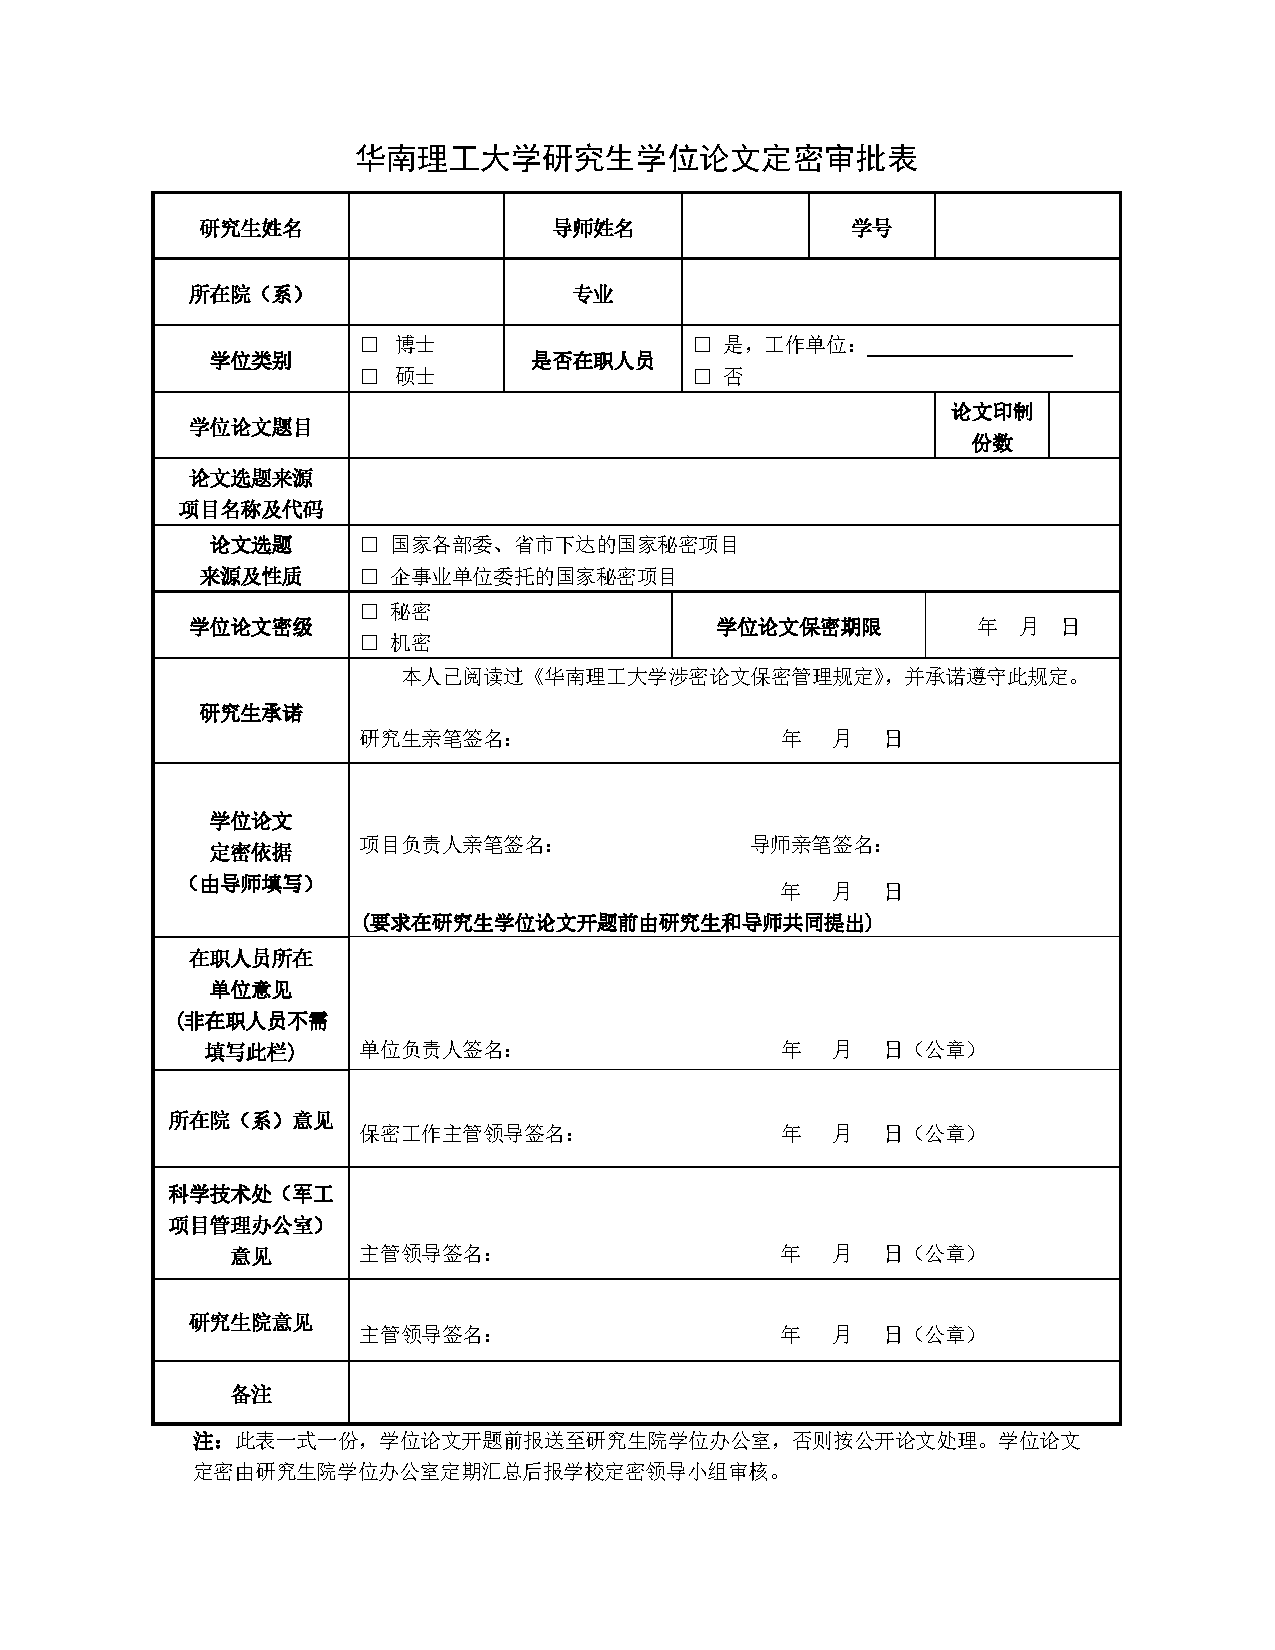
\includepdf[pages={1}]{final.pdf}
\end{document}